\section{RNN}
\label{sec:part-rnn}

\subsection{Model Training}

We utilised \textit{Weights \& Biases Agent}\footnote{Documents available in \url{https://docs.wandb.ai/guides/sweeps}} to track and sweep the best model hyperparameter. Bayesian Optimization \cite{dewancker2016bayesian} is used as the strategy to sweep the best hyperparameter. By default, we set the \textit{require\_grad} for word embedding to False to freeze the parameters. We use the simple RNN design with PyTorch~\citep{paszke2019pytorch} that takes each token as hidden states and iterative to the final token for each sequences.

\subsection{Best model}

Due to computational and time limit, we can only run limited experiments. We employ two search strategies, \textbf{1)} Grid Search, \textbf{2)} Manually tuned. The config and the search space is listed in Table \ref{tab:best_model_config}. However, we find out that one of the config when manually tuned the parameters reaches the best result and we adopt that setting as our best model config

\begin{table}[ht]
    \centering
    \begin{tabular}{c | c | c}
    \toprule
    \textbf{Config} & \textbf{Value} & \textbf{Grid Search Space}\\
    \midrule
    Layer & $5$ & $\{3,4,5,6\}$\\
    Input Dim & $300$ & -\\
    Hidden Dim & $512$ & - \\
    \midrule
    Optimizer & AdamW & - \\
    LR Scheduler & \texttt{CosineAnnealingLR} & - \\
    Warmup Ratio & 0.03 & - \\
    Learning Rate & $1.63\times 10^{-5}$ & $1 \times 10^{-3} \sim 1 \times 10^{-5}$\\
    Weight Decay & $0.4$ & - \\
    Batch Size & $4 \text{ (GPUs)}\times 8$ & $4\times \{8, 16, 32\}$\\
    \bottomrule
    \end{tabular}
    \caption{Best Model Config}
    \label{tab:best_model_config}
\end{table}

We also present our grid search results in~\cref{fig:sweep} for multiple trials and use the best model config that achieve the highest evaluation accuracy.

\begin{figure}[h]
    \centering
    \centering
    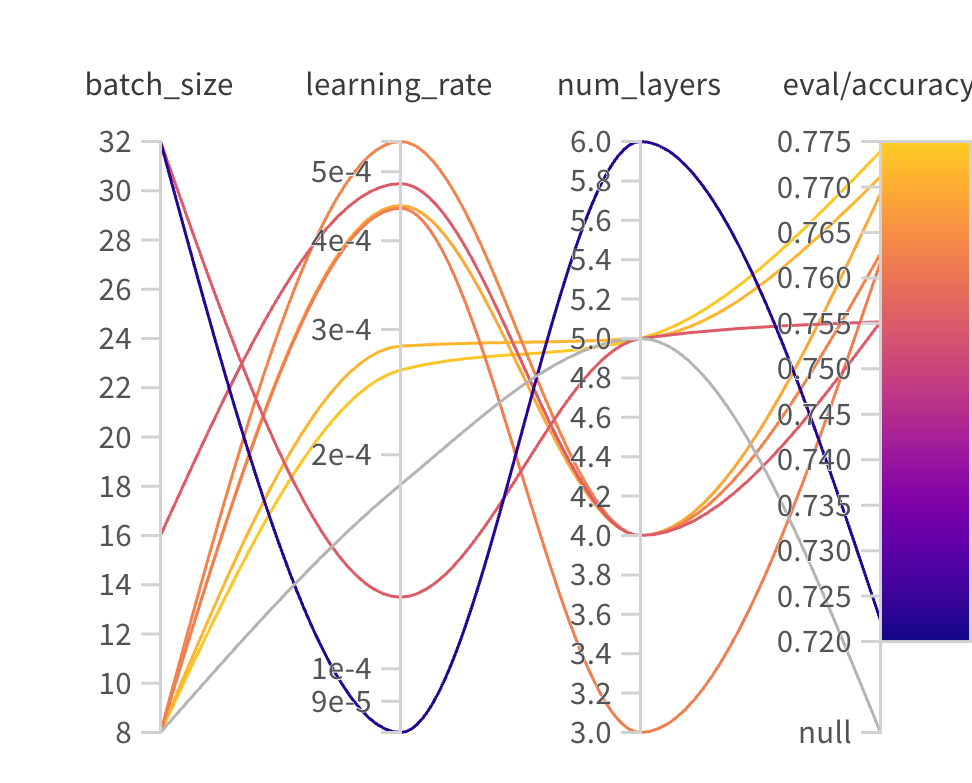
\includegraphics[width=0.85\linewidth]{images/sweep.png}
    \caption{Sweep result}
    \label{fig:sweep}
\end{figure}



\subsection{Model Performance}

\begin{table}[ht]
    \centering
    \begin{tabular}{c | c | c | c}
    \toprule
    \textbf{Metric} & \textbf{Train set} & \textbf{Validation set} & \textbf{Test set}\\
    \midrule
         \textbf{Loss} & $0.5619$ & $0.5228$ & $0.5416$\\
         \textbf{Accuracy} & - & $77.86\%$ & $76.27\%$\\
    \bottomrule
    \end{tabular}
    \caption{Performance table}
    \label{tab:performance}
\end{table}

Our model's performance, as shown in Table~\ref{tab:performance}, is evaluated across the training, validation, and test sets using both loss and accuracy metrics. The loss values are 0.5619, 0.5228, and 0.5416 for the training, validation, and test sets, respectively, indicating consistent performance with slight variations across the datasets. The model achieves an accuracy of 77.86\% on the validation set and 76.27\% on the test set, suggesting that it generalizes well to unseen data with minimal overfitting.

\paragraph{Setting} We use the same settings to run all the experiments with batch size equals to 8 and learning rate equals to $1 \times 10^{-5}$. For every run, we train 10 epochs and report the final validation and test result.

\subsection{Sentence Representation Methods}

\begin{table}[h]
\centering
\caption{The result of using different sentence representation strategies}
\label{tab:sentence}
\begin{tabular}{l|llll}
\toprule
Aggregation & Test/Acc      & Test/Loss     & Val/Acc       & Val/Loss      \\
\midrule
Average     & 0.72          & 0.63          & 0.73          & 0.63          \\
Sum         & \textbf{0.76} & \textbf{0.56} & \textbf{0.76} & \textbf{0.55} \\
Final Token & 0.51          & 0.69          & 0.50          & 0.69         
\end{tabular}
\end{table}

We compare three sentence representation methods—average, sum, and final token—using accuracy and loss metrics on both the validation and test sets. As shown in Table~\ref{tab:sentence}, the sum aggregation method achieves the best performance, with a test accuracy of 0.76 and a test loss of 0.56. This method also yields a validation accuracy of 0.76 and a validation loss of 0.55, outperforming both the average and final token methods. The average method yields moderate results, with a test accuracy of 0.72 and validation accuracy of 0.73, while the final token method shows the lowest performance across all metrics. These results indicate that summing embeddings captures sentence information most effectively in our RNN model, supporting our decision to use this method as the default aggregation strategy.

